\chapter{Energy}
\section{Kinetic Energy and Work}
The simplest form of energy is \textbf{kinetic energy} (or KE), which is defined for a particle of mass $m$ moving at velocity $\mbf{v}$ to be
\[ T = \frac{1}{2}m (\mbf{v}\cdot\mbf{v}) = \frac{1}{2}mv^2 =  \]
Imagine the particle moving through space and examine the object's change in kinetic energy as it moves between two neighboring points $\mbf{r}_1$ and $\mbf{r}_1 + \dd \mbf{r}$.  We can differentiate $T$ with respect to time with the product rule for the dot product
\[ \dv{T}{t} = \frac{1}{2}m (\mbf{\dot v} \cdot \mbf{v} + \mbf{v}\cdot\mbf{\dot v}) = m(\mbf{\dot v}\cdot \mbf{v})\]
By Newton's second law $\mbf{F} = m\mbf{\dot v}$, so
\[ \dv{T}{t} = \mbf{F} \cdot \mbf{v} \]
multiplying both sides by $\dd t$ and noting that $\mbf{v}\dd t = \dd\mbf{r}$,
\[ \dd T = \mbf F \cdot \dd \mbf{r} \]
We define the expression $\mbf{F}\cdot \dd\mbf{r}$ as the work done by $\mbf{F}$ as the object undergoes displacement $\dd\mbf{r}$. Thus, the change in a particle's kinetic energy between two neighboring points on its path is equal to the work done by the net force on the particle as it moves between the two points. This is known as the Work-KE theorem.

So far, we've only proven the Work-KE theorem for two infinitesimally close points, but it is relatively simple to generalize to larger displacements. Consider two points $A$ and $B$ with position vectors $\mbf{a}$ and $\mbf{b}$. Suppose a particle follows some path arbitrary path $C$ from $\mbf{a}$ to $\mbf{b}$. We can find the total change in kinetic energy by splitting $C$ into many infinitesimal curves and summing the work across each of them.
\[ \Delta T \equiv T_A - T_B = \lim_{n\to\infty} \sum_{i=1}^n \mbf{F}\cdot \dd \mbf{r_i} \]
this limit can be recognized as approaching the value of the line integral
\[ \Delta T = \int\limits_C \mbf{F}\cdot\dd\mbf{r} \]
as $n\to\infty$. We may also use the alternative notation $\Delta T = \int_A^B\mbf{F}\cdot\dd\mbf{r}$ to represent the same quantity. 

I will also introduce the notation $\int_A^B \mbf{F}\cdot\dd\mbf{r} = W(A\to B)$ to represent the work done as an object moves from $A$ to $B$. 

Another useful property of our definition of work is that the work done by the net force $\mbf{F} = \mbf{F}_1 + \cdots + \mbf{F}_n$ is equal to the sum of the works done by each $\mbf{F}_i$. This result is fairly easy to show.
\begin{align*}
    W(A\to B) &= \int_A^B \mbf{F}\cdot\dd\mbf{r} = \int_A^B \sum_i \mbf{F}_i \cdot \dd \mbf{r} \\
    &= \sum_i \int_A^B \mbf{F}_i \cdot \dd \mbf{r} = \sum_i W_i(A\to B)
\end{align*}
the step between the first and second line is justified by the linearity of the integral. This allows us to write
\begin{equation}\label{workthm}
    \Delta T = \sum_i W_i(A\to B)
\end{equation}
When using the Work-KE theorem, we almost always use it in the form (\ref{workthm})--calculate the work $W_i$ from each individual force acting on the particle, and then set $\Delta T$ equal to their sum. 
\section{Potential Energy and Conservative Forces}
For now, assume that there is just one force acting on the object of interest--this may be the gravitational force between an object and a planet, the electrostatic force on a charged particle in an electric field, an applied force, or really anything else. Depending on the force, it may depend on several different attributes of the object; its velocity, position, time, etc.

We will draw our attention to a particular classification of forces, called \textit{conservative forces}. The properties of these forces will soon become apparent. For a force to be conservative, the first criteria is that it must be solely dependent on the position $\mbf{r}$. For instance, the gravitational force can be written as a function of $\mbf{r}$,
\begin{equation} \label{gforc}
    \mbf{F}(\mbf{r}) = -\frac{GmM}{r^2}\rhat = -\frac{GmM\mbf{r}}{\abs{\mbf{r}}^3}
\end{equation}
Similarly, the electrostatic force on a particle with a non time-dependent electric field is given by $\mbf{F}(\mbf{r}) = q\mbf{E}(\mbf{r})$.

The second condition for a force to be conservative is that the work done between two points $A$ and $B$ must be identical regardless of the path taken between $A$ and $B$. For an example of a force that does not follow this rule, consider the force of friction on an object sliding across the ground. The force is given by
\[ \mbf{F}_\text{fric} = -\mu_k F_N \mbf{\hat v} \]
Because $\dd\mbf{r} = \mbf{v}\dd t$, $\dd \mbf{r}$ is parallel to $\mbf{\hat v}$ and the work is given by
\[ W_\text{fric} = -\mu_k F_N \int_A^B \dd s = -\mu_k F_N \ell \]
where $\ell$ is the length of the path taken from $A$ to $B$. Because two different paths may have different lengths, the work done due to friction is not independent of path, and so friction is not a conservative force. 

For an example of a force that is independent of path, consider the gravitational force. (\ref{gforc}) gives us an expression for $\mbf{F}_\text{grav}$ in terms of $\mbf{r}$. Then,
\begin{align*}
    W_\text{grav} &= -GmM \int_A^B \frac{\mbf{r}}{r^3}\cdot \dd \mbf{r}
\end{align*}
recall from Multivariable Calculus that a line integral is independent of path if and only if the curl of the integrand is $\mbf{0}$. This is true for the gravitational force, as you should verify. 

The name conservative comes from the property that if all forces on the object are conservative, we can define a quantity called the potential energy (PE), denoted $U(\mbf{r})$, a function of only position, with the property that the total mechanical energy
\[ E = T + U(\mbf{r}) \]
is constant. This is known as the principle of conservation of energy, and we will see  how it naturally arises from the below definition of $U$. 

To define the potential energy $U(\mbf{r})$ corresponding to a given conservative force, first choose some reference point $\mbf{r}_0$ where $U$ is defined to be zero. For example, when we analyze gravity near the surface of the Earth, we often define $U$ as zero at ground level. Then, the potential energy at some $\mbf{r}$ is given by
\[ U(\mbf{r}) = -W(\mbf{r}_0\to\mbf{r}) = -\int_{\mbf{r_0}}^{\mbf{r}} \mbf{F}(\mbf{r}')\cdot \dd \mbf{r}' \]
Notice that this definition only makes sense due to the fact that $\mbf{F}$ is conservative--otherwise, we could get several different values for $U(\mbf{r})$ by taking different paths. We will see the reason for the minus sign shortly. 
\begin{example}[Potential Energy of a Charge in a Uniform Electric Field]
    Suppose a charge $q$ is placed in a uniform electric field $\mbf{E} = E_0\xhat$ so that the electric force on $q$ is given by $\mbf{F} = qE_0\xhat$. Show that this force is conservative and find the corresponding potential energy as a function of the position $\mbf{r}$ of the charge. Assume that the gravitational force is negligible.

    The work done by $\mbf{F}$ going between any two points $A$ and $B$ along any path is given by
    \begin{equation} \label{elecconsrv}
        W(A\to B) = \int_A^B \mbf F \cdot \dd \mbf r = qE_0 \int_A^B \xhat \cdot \dd \mbf r = \int_A^B \dd x = qE_0(x_B - x_A)
    \end{equation}
    Because ($\ref{elecconsrv}$) has the same value regardless of the path taken from $A$ to $B$, $\mbf{F}$ is conservative. To define a potential energy, we must define some point where $U=0$. The obvious choice is the origin $\mbf r_0 = \mbf 0$, so
    \[ U(\mbf{r}) = -W(\mbf 0 \to \mbf{r}) = -qE_0 r_x\]
\end{example}

Another critical result can be derived by considering a conservative force $\mbf{F}$ and three points $\mbf{r}_0$, $\mbf{r}_1$, $\mbf{r}_2$, where we define $\mbf{r}_0$ as the reference point where $U(\mbf{r}_0) = 0$. It is easy to convince yourself that
\[ W(\mbf{r}_0 \to \mbf{r}_2) = W(\mbf{r}_0 \to \mbf r_1) + W(\mbf r_1 \to \mbf r_2) \]
which can be rearranged to obtain
\[W(\mbf r_1 \to \mbf r_2) = W(\mbf r_0 \to \mbf r_2) - W(\mbf r_0 \to \mbf r_1)\]
But since $\mbf r_0$ is our reference point, this simply becomes
\[ W(\mbf r_1 \to \mbf r_2) = -(U(\mbf r_2) - U(\mbf r_1)) = -\Delta U \]
This is particularly useful when we combine it with the Work-KE theorem, giving
\[ \Delta T = -\Delta U\]
or
\[ \Delta T + \Delta U = 0\]
In other words, the total mechanical energy $E = T + U$ is conserved. 
\subsection*{Several Forces}
So far we have established the conservation of energy for a particle subject to a single conservative force. We will now see that this result generalizes nicely to an object subject to several conservative forces. For instance, consider a mass suspending from the ceiling by a spring. There are two forces present on the object, the force of gravity $\mbf{F}_\text{grav}$ and the spring force $\mbf{F}_\text{spr}$. As we've already shown, the gravitational force is conservative, and it is relatively easy to see that the force of a spring that obeys Hooke's Law is conservative as well. 
\begin{align*}
    \curl (-k\mbf{r}) = -k (\curl{\mbf r}) = \mbf 0  
\end{align*}
The Work-KE theorem tells us that
\begin{align*}
    \Delta T &= W_\text{grav} + W_\text{spr} \\
    &= -(\Delta U_\text{grav} + \Delta U_\text{spr})
\end{align*}
Rearranging, we obtain $\Delta T + \Delta U_\text{grav} + \Delta U_\text{spr} = 0$, showing that the total mechanical energy of the system is conserved. Similar arguments follow for an arbitrary number of conservative forces.
\begin{theorem}[Principle of Conservation of Energy on a Particle]
    If all of the $n$ forces $\mbf{F}_1, \dots, \mbf{F}_n$ acting on a particle are conservative with a corresponding potential energy $U_1(\mbf{r}), \dots, U_n(\mbf{r}) $, then the total mechanical energy
    \[ E = T + U_1(\mbf{r}) + \cdots + U_n(\mbf{r}) \] 
    is constant.
\end{theorem}
\subsection*{Nonconservative Forces}
If some of the forces on the particle are nonconservative, then we cannot define corresponding potential energies, and we cannot define a conserved mechanical energy. To remedy this, we will split the forces on the object based on whether they are conservative or nonconservative, and we will define the total work done on the object as
\[ W = W_\text{cons} + W_\text{nc}\]
where $W_\text{cons}$ is the work done by all of the conservative forces and $W_\text{nc}$ is the work done by all of the nonconservative forces. This also gives
\[ \Delta T = W_\text{cons} + W_\text{nc} = -\Delta U + W_\text{nc} \]
This can be rearranged to obtain $\Delta T + \Delta U = W_\text{nc}$, or simply $\Delta E = W_\text{nc}$. 

So although mechanical energy is not conserved, it only changes by the amount of work done by all of the nonconservative forces.
\begin{example}[Inclined Plane With Friction]
    Consider a block that starts at rest and begins to slide down a rough incline of angle $\theta$ and coefficient of kinetic friction $\mu_k$.Find the speed $v$ of the object after it as traveled a distance $d$ along the slope. 

    As in the previous inclined plane example (\ref{inclined}), we set up the unit vectors such that $\xhat$ points down the incline and $\yhat$ points normal to the incline. Then, the three forces on the object are 
    \begin{align*}
        \mbf{F} &= \mbf{F}_N + \mbf{F}_\text{grav} + \mbf{F}_\text{fric} \\
        &= (N - mg\cos\theta)\yhat + (mg\sin\theta - \mu_k N)\xhat
    \end{align*}
    Because the net force in the $\yhat$ direction must be zero, we have $N = mg\cos\theta$ and therefore $F_\text{fric} = \mu_k mg \cos \theta$. The gravitational force conservative with potential energy $U = mgh$, where $h$ is the vertical difference between the height where $U=0$ and the current height. We will take $U=0$ to be at the final $h$ value, after the object has slid a distance $d$.

    Through basic trigonometry, this tells us that the height of the initial position of the block relative to the final position is $h_0 = d\sin\theta$, and therefore
    \[ \Delta U = -mgd\sin\theta \]
    
    The normal force does not do any work on the particle (as it is perpendicular to the velocity which solely points in the $\xhat$ direction).  

    Because the frictional force is always antiparallel to the velocity vector, we have
    \[ W_\text{nc} = W_\text{fric} = -\mu_k dmg\cos\theta \]
    Finally, the kinetic energy of the particle is simply $T = \frac{1}{2}mv^2$, as always. Because the object is initially at rest, the initial kinetic energy is zero and $\Delta T = T$. Then, since $\Delta T + \Delta U = W_\text{nc}$, we have
    \[ \frac{1}{2}mv^2 - mgd\sin\theta = -\mu_k dmg\cos\theta \]
    which can be rearranged to find
    \[ v = \sqrt{2gd(\sin\theta-\mu_k \cos\theta)}\]
\end{example}
\section{Force as the Gradient of Potential Energy}
Previously, we wrote the potential energy $U(\mbf{r})$ of a particle undergoing conservative forces as a type of integral of the force $\mbf{F}(\mbf{r})$. Now, it seems natural to write the force as some form of derivative of the potential energy. To begin, the change in potential energy as an object moves from $\mbf r$ to $\mbf r + \dd \mbf r$ is, by definition
\[ \dd U = U(x + \dd x, y + \dd y, z + \dd z) - U(x, y, z) \]
Just as we can write $f(x + \dd x) - f(x) = \dv{f}{x}\dd x$ for functions of a single variable, we can write
\begin{align}
    \dd U &=  U(x + \dd x, y + \dd y, z + \dd z) - U(x, y, z) \nonumber \\
    &= \pdv{U}{x}\dd x + \pdv{U}{y}\dd y + \pdv{U}{z}\dd z \label{du1}
\end{align}
We can also write 
\begin{align}
    \dd U &= -\int_{\mbf r}^{\mbf r + \dd r} \mbf{F}(\mbf{r}') \cdot \dd \mbf{r}' \approx -\mbf{F}(\mbf{r})\cdot \dd \mbf{r} \nonumber \\
    &= -\pqty{F_x\dd x + F_y\dd y + F_z\dd z } \label{du2}
\end{align}
By equating (\ref{du1}) and (\ref{du2}), we obtain
\[ \pqty{\pdv{U}{x} + F_x}\dd x + \pqty{\pdv{U}{y} + F_y}\dd y + \pqty{\pdv{U}{z} + F_z}\dd z = 0\]
To simplify this equation somewhat, imagine the special case where the object is only moving in the $x$ direction; in other words, $\dd y = \dd z = 0$. This gives $F_x + \partial U/\partial x = 0$ or $F_x = -\partial U/\partial x$. Repeating this process for the $y$ and $z$ coordinates, we find
\[ F_x = -\pdv{U}{x} \quad F_y = -\pdv{U}{y} \quad F_z = -\pdv{U}{z} \]
In vector form, this equation can be simply written as 
\[ \mbf{F} = -\nabla U \]
One thing to note is that this whole analysis hinges upon the fact that $\mbf{F}$ is conservative. In other words, conservative forces are always derivable from a potential energy. 
\begin{example}[Finding a Force From a Potential Energy]
    The potential energy of a particle is given by $U = Axy^2 + B\sin Cz$ where $A,B,C\in\R$ are arbitrary. Find the corresponding force field.
    
    To find $\mbf{F}$, we simply compute the gradient of $U$ and multiply it by $-1$.
    \[ \mbf{F} = -\nabla U = -Ay^2\xhat - 2Axy\yhat - BC\cos(Cz)\zhat \]
\end{example}
Another useful relationship that we will take advantage of is the fact that
\[ \dd U = \nabla U \cdot \dd \mbf{r} \]
This is a general property of the gradient that we may also apply in other scenarios as well.
\section{Time-Dependent Potential Energy}
Consider a force $\mbf{F}(\mbf{r}, t)$ that satisfies $\curl\mbf{F} = \mbf 0$. This field is still conservative in the mathematical sense--there exists some potential $U(\mbf{r},t)$ such that $\mbf F = -\nabla U$. But because there is a time dependency, it is no longer the case that the total mechanical energy $E = T + U$ is conserved.

As a sidenote, the $\nabla$ operator is still defined as $\langle \partial_x, \partial_y, \partial_z \rangle$ when working with time-dependent fields--that is, we only consider the spatial coordinates in operations involving $\nabla$.

For an example of a field of this type, consider a conducting sphere with a non-constant charge $Q(t)$--for instance, suppose the sphere is connected by a rod with non-negligible resistance to the ground, causing charge to slowly leak into the ground.

It is relatively easy to show that the force $\mbf{F}_\text{elec}$ exerted on a small charge $q$ is non-constant, but satisfies $\curl \mbf{F}_\text{elec}(\mbf r, t) = \mbf 0$ for all $\mbf{r}$ and $t$. 

To show that a potential energy function indeed exists, recall that $\curl\mbf{F}(\mbf r, t) = 0$ tells us that any line integral of $\mbf{F}$ is dependent only on the endpoints (path independence). Therefore, we can define $U(\mbf{r}, t)$ as
\[ U(\mbf{r},t) = -\int_{\mbf{r_0}}^{\mbf{r}} \mbf{F}(\mbf{r}', t)\cdot \dd \mbf{r}' \]
where $\mbf{r}_0$ is some sample point where we define $U(\mbf{r}, t) =0$. Using the same methods as in the previous section, we can show that $\mbf{F}(\mbf{r}, t) = -\nabla U(\mbf{r}, t)$.

So far, everything is identical to the behavior of $U$ with no time dependence, but now the story changes. We define the total mechanical energy $E = T + U$, as usual. Consider two nearby points in time $t$ and $t + \dd t$. The change in kinetic energy $T$ is given by
\begin{align} \label{dt,td}
    \dd T = \dv{T}{t}\dd t = m(\mbf{\dot v} \cdot \mbf{v})\dd t = \mbf{F}\cdot \dd \mbf{r} 
\end{align}
and the change in potential energy $U$ is given by
\[ \dd U = \pdv{U}{x}\dd x + \pdv{U}{y}\dd y + \pdv{U}{z}\dd z + \pdv{U}{t}\dd t \]
The first three terms on the left can be recognized as $\nabla U \cdot \dd \mbf{r} = -\mbf{F}\cdot\dd\mbf{r}$. Therefore,
\begin{equation} \label{du,td}
    \dd U = -\mbf{F}\cdot\dd\mbf{r} + \pdv{U}{t}\dd t
\end{equation}
The total change in mechanical energy is the sum of (\ref{dt,td}) and (\ref{du,td}):
\[ \dd E = \pdv{U}{t}\dd t\]
Clearly, the mechanical energy $E$ is only conserved when $U$ is independent of $t$; that is, when $\partial U/\partial t = 0$. 

\section{Energy in Linear One-Dimensional Systems}
So far we have only discussed energy for a particle that is free to move in all three spatial dimensions. Many interesting and important problems involve an object that is constrained to move in just one dimension, and the methods to analyze these problems is much simpler than the more general case. 

We are used to the notion of a one-dimensional system as a perfectly straight, or linear, track. In discussing these types of linear systems, we take the $x$ axis to coincide with the track, and the position of the object is specified by a single coordinate $x$. There are much more complicated linear systems, however. Consider a roller coaster following a track; the system is still one dimensional, although it is not linear.

In this section, we will focus solely on linear one-dimensional systems, although we will soon see that analysis of nonlinear one-dimensional systems does not differ from analysis of their linear counterparts as much as one might expect.

To begin, consider an object constrained to move along a perfectly straight track, which we take to be the $x$ axis. The only component of any force $\mbf{F}$ that can do any work is the $x$ component, and so we can simply ignore the other components. Thus, the work is given by
\begin{equation} \label{work1d}
    W(x_1\to x_2) = \int_{x_1}^{x_2} F_x(x)\; \dd x
\end{equation}
As before, for $F_x$ to be conservative, it must satisfy the following two conditions:
\begin{enumerate}
    \item The force $F_x$ depends only on the position $x$.
    \item The integral (\ref{work1d}) is independent of path.
\end{enumerate}
For one-dimensional systems, however, the first condition implies the second so the second condition can be disregarded altogether.

For the first condition, notice that despite the fact that we are in one dimension only, there are still many possible paths from $x_1$ to $x_2$. There is, of course, the straight path that takes us directly from $x_1$ to $x_2$. But then, consider another path that goes from $x_1$ to $x_2$ and then \textit{continues} going to another point $x_3$ that is past $x_2$, before doubling back and returning to $x_2$. The work done along this path is described by
\[ W(x_1\to x_2 \to x_3\to x_2) = W(x_1\to x_2) + W(x_2\to x_3) + W(x_3\to x_2) \]
Provided the force $F_x$ is only dependent on the position $x$, we have
\begin{align*}
    W(x_3\to x_2) &= \int_{x_3}^{x_2}F_x(x)\; \dd x = -\int_{x_2}^{x_3} F_x(x) \; \dd x = -W(x_2\to x_3)
\end{align*}
Thus the $W(x_2\to x_3)$ and $W(x_3\to x_2)$ terms cancel and we simply have
\[ W(x_1\to x_2\to x_3 \to x_2) = W(x_1\to x_2)\]
These same principles can be applied to paths that double back on themselves arbitrarily many times before finally reaching their final destinations, showing that the work is fully independent of path. 
\subsection*{Graphs of the Potential Energy}
A second useful feature of one-dimensional system is that we can graph the potential energy $U(x)$ as a function of only one variable, making visualization a much easier task than it would be in several dimensions.

Assuming all forces acting on an object are conservative, we can write
\[ U(x) = U(x_0)-\int_{x_0}^x F_x(x')\; \dd x'\]
We often choose $x_0$ such that $U(x_0) = 0$, causing the left term to go away.

For instance, if a mass is attached to a spring obeying Hooke's Law, we have $F_x(x) = -kx$, so choosing $x_0=0$ to be the location with zero potential energy,
\begin{align*}
    U(x) &= -\int_0^x F_x(x')\; \dd x' \\
    &= k\int_0^x x' \; \dd x' = \frac{1}{2}kx^2 
\end{align*}
The one-dimensional analogue to the relationship $\mbf{F} = -\nabla U$ is the comparatively simple result
\[ F_x = -\dv{U}{x} \]

Plotting the potential energy against $x$ allows us to qualitatively analyze how the object must behave. The direction of the net force is the opposite of the slope of the graph of $U(x)$, so the object will naturally tend to accelerate ``downhill" on the graph.
\begin{figure}[h!]
    \centering
    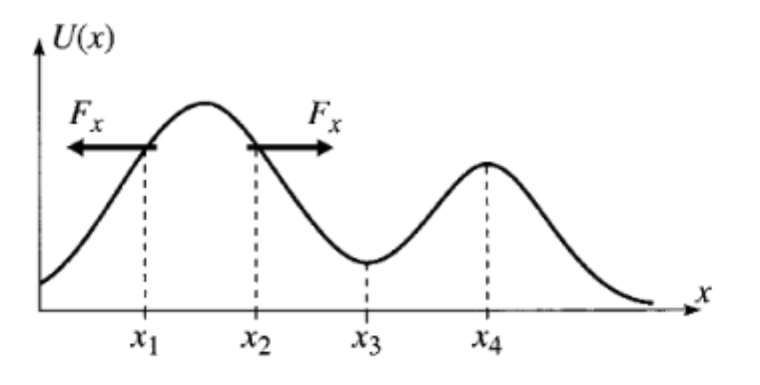
\includegraphics[width=0.5\linewidth]{potentialEnergy1d.png}
    \label{fig:U1d}
\end{figure}
At locations such as $x_3$ and $x_4$ where the graph has an extremum, the net force on the object is zero and so the object may remain in equilibrium there (provided it is initially stationary). Depending on whether the extrema is a local minimum or maximum, we call it either a \textit{stable equilibrium} (local minimum) or an \textit{unstable equilibrium} (local maximum). To justify this, imagine an object stationary at a stationary equilibrium such as $x_3$ on the above graph. If it receives a small perturbation in either direction, it will tend to accelerate back towards the equilibrium point. If it were instead at an unstable equilibrium such as $x_4$ on the above graph, a small perturbation would cause the object to continually accelerate away from the equilibrium point.

Some graphs may have an extremum that is stable in one direction and unstable in the other--we call these \textit{semi-stable equilibrium} points. These are rarer than stable or unstable equilibrium points, but one example would be at $x=0$ if we had $U(x) = x^3$.

We can also study these objects' behavior with the conservation of energy. Suppose at some point $x=x_0$, we have
\[ E = T(x_0) + U(x_0) \]
Because $E$ is constant, we then necessarily have, for any point $x_1$,
\[ T(x_1) + U(x_1) = T(x_0) + U(x_0) \]
Suppose that $x_1 > x_0$ and there exists some $b$ such that $x_0 < b < x_1$ and
\[ U(b) = T(x_0) + U(x_0) \]
Then, it is \textit{impossible} for the object to pass $x = b$ without an external force, as that would require it to possess some kinetic energy there. But we know this cannot be the case, as 
\[ U(b) + T(b) = T(x_0) + U(x_0)  \]
implying $T(b) = 0$. In this case, we call $x=b$ a \textit{turning point} for the motion of the object, provided it is not an equilibrium point, as it causes the object to turn around and begin accelerating in the opposite direction.

One insightful way to visualize the locations of these turning points is to draw a horizontal line at $U(x) = E$, such as the graph below.
\begin{figure}[h!]
    \centering
    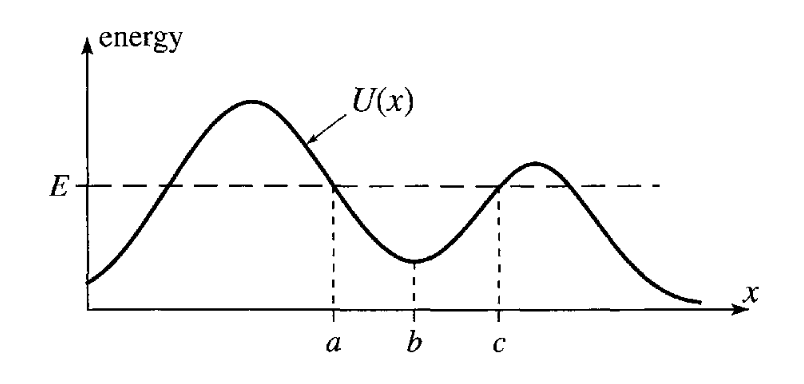
\includegraphics[width=0.5\linewidth]{potentialEnergy1d_2.png}
    \label{fig:U1d2}
\end{figure}

any point above the dashed horizontal line cannot be reached without some non-conservative force increasing the total energy of the particle (this is unlikely, as non-conservative forces typically dissipate energy rather than increase it).

Further, if the object ever enters the area between $x=a$ and $x=c$, it will continue to oscillate between them indefinitely--it can never escape this ``well" as that would require it have enough energy to overcome the crest of the hills on either side, which it simply doesn't. If the object has enough energy to overcome the crest on the right side, but not the crest on the left side, we can guarantee that it will escape to the right. If it has enough energy to overcome both crests, it could escape in either direction.
\subsection*{Complete Solution of the Motion}
Another remarkable feature of one-dimensional conservative systems is that we can use the conservation of energy to obtain a complete solution of the motion, as long as we know the total energy $E$ and the potential energy $U(x)$.

The equation $\frac{1}{2}m\dot{x}^2 + U(x) = E$ can be rearranged to give
\[ \dot x = \pm \sqrt{\frac{2}{m}(E-U(x))}\]
The sign ambiguity comes from the fact that kinetic energy is the same regardless of the direction of $\dot x$. 

This is a first order autonomous differential equation that can be solved through separation of variables, giving

\[ \sqrt{\frac{m}{2}}\int_{x_0}^x \frac{\dd x'}{\sqrt{E-U(x)}} = t - t_0\]
where $x(t_0) = x_0$.
\section{Curvilinear One-Dimensional Systems}
We will now turn our attention to the other type of linear system I mentioned--systems where the path may not be straight.

Instead of defining the position in terms of a distance $x$ along an axis, we will define it in terms of an arc-length $s$ along the curve. To develop equations describing the path, we will consider two frameworks to analyze its motion. First, there is the one dimensional perspective we have just laid out, where position is measured in terms of the arclength $s$. However, we can also talk about the position of the particle in terms of its $x$ and $y$ components. These systems are related with the line integral 
\[ s = \int\limits_C \dd s'\]
Where $C$ is the curve going from the point we have denoted $s=0$ to the point at which we are measuring $s$. We can also write
 \[ \dd s = \sqrt{\dd x^2 + \dd y ^2} \]
 or
 \[ \dot s = \sqrt{\dot x^2 + \dot y^2}\]
 Recognizing $\sqrt{\dot x^2+\dot y^2}$ as the speed of the particle, this tells us that in terms of arclength, the speed is simply $\dot s$. We can then write the kinetic energy as
\[ T = \frac{1}{2}m\dot s^2\]
As for the force, we will consider it as the sum of a normal component and a tangential component. The normal component is often called the \textit{force of constraint} as it is what causes the particle to remain on the path--if we consider osculating circle to the curve, we can imagine the normal component as a type of centripetal force keeping the object along the ever-changing circular path. 

Because the normal component is perpendicular to the path of the particle, it does no work on it. Further, we have $m\ddot{s} = F_\text{tan}$. To show this, first note the relationship $v^2 = \dot s^2 = \mbf{v} \cdot \mbf{v}$. Taking the time derivative of each side, we find
\begin{align*}
    \dot{s}\ddot{s} = \mbf{v} \cdot \mbf{\dot v}
\end{align*}
if we write the net force vector as 
\[ \mbf{F} = F_\text{tan}\mbf{\hat{T}} + F_\text{N} \mbf{\hat N}\]
where $\mbf{\hat{T}}$ is the unit tangent vector to the curve and $\mbf{\hat{N}}$ is the unit normal vector to the curve, we get
\[ \mbf{\dot v} = \frac{1}{m} (F_\text{tan}\mbf{\hat{T}} + F_\text{N} \mbf{\hat N}) \]
or
\[ m\dot{s}\ddot{s} = F_\text{tan}\mbf{v} \cdot \mbf{\hat{T}} + F_\text{N} \mbf{v}\cdot \mbf{\hat N} \]
Because the velocity is always parallel to the tangent vector and orthogonal to the normal vector, $\mbf{v}\cdot\mbf{\hat T} = v = \dot s$ and $\mbf{v}\cdot\mbf{\hat N} = 0$. Therefore,
\[ m\ddot{s} = F_\text{tan}\]
as desired. 

If all of the forces on the particle with a tangential component are conservative, we can define a potential energy $U(s)$ with
\[ U(s) = \int_{s_0}^s F_\text{tan}(s')\; \dd s'\]
similar to the potential energy in linear one-dimensional systems, we have $F_\text{tan} = -\dd U/\dd s$ and we can apply the entirety of our previous discussion about the graphs of $U$ to curvilinear coordinates without many changes.

\begin{example}[Stability of a Cube Balanced on a Cylinder]
    
    \begin{minipage}{0.48\textwidth}
        A hard rubber cylinder of radius $r$ is held fixed with its axis horizontal, and a cube of mass $m$ and sidelength $2b$ is balanced on top of the cylinder, with its center vertically about the cylinder's axis and four of its sides parallel to the axis. The cube cannot slip on the rubber of the cylinder, but it can rock from side to side. Determine if the equilibrium of the cube centered above the cylinder is stable. 

        This system seems complicated, but it is in fact a one-dimensional system in terms of the angle $\theta$ formed between the vertical and the side of the box pointing up. The forces acting on the box are the normal force between it and the cylinder and the gravitational force acting on the box. If we define $h=0$ to be at the height of the axis of the cylinder, we know that the gravitational potential energy is given by $U = mgh$.
    \end{minipage}
    \begin{minipage}{0.48\textwidth}
        \parbox{\textwidth}{
            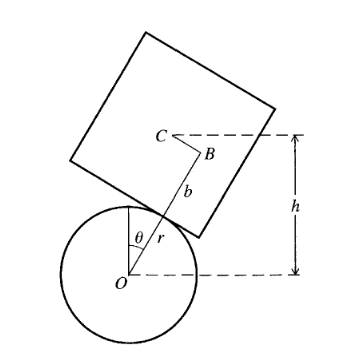
\includegraphics[width=\textwidth]{cubeOnCylinder.png}
        }
    \end{minipage}
    
    With some geometry, we can see that
    \[ h = (r+b)\cos\theta + r\theta\sin\theta \]
    The $r\theta\sin\theta$ term originates from the fact that the length of the line segment $BC$ is the amount the cube has rolled down the cylinder, namely $r\theta$, and the component of that in the vertical direction is $r\theta\sin\theta$.

    Therefore the potential energy as a function of $\theta$ is given by
    \[ U(\theta) = mg((r+b)\cos\theta + r\theta\sin\theta) \]
    and its derivative is 
    \begin{align*}
        \dv{U}{\theta} &= mg(r\sin\theta + r\theta\cos\theta - (r+b)\sin\theta) \\
        &= mg(r\theta\cos\theta - b\sin\theta) 
    \end{align*}
    Equilibrium occurs at the point where $\dd U/\dd \theta = 0$, or when $r\theta\cos\theta = b\sin\theta$. The nonzero solutions to this equation cannot be found analytically, and whether or not a nonzero solution even exists will depend on the $b$ and $r$ values. For the solution where $\theta = 0$, however, we can determine the stability with the second derivative test.
    \begin{align*}
        \dv[2]{U}{\theta} = mg((r-b)\cos\theta - r\theta\sin\theta)
    \end{align*}
    and when $\theta =0$,
    \[ \dv[2]{U}{\theta}\biggr|_{\theta = 0} = mg(r-b)\]
    Therefore the equilibrium at $\theta = 0$ is stable if $r > b$ and unstable if $r < b$. If $r=b$, the second derivative reduces to
    \[ \dv[2]{U}{\theta} = -r\theta\sin\theta\]
    and the second derivative test is inconclusive. We will have to differentiate again (twice, actually--the third derivative turns out to be zero as well) to find that $\theta = 0$ is an unstable equilibrium. 
\end{example}
\subsection*{Further Generalizations}
Many other complicated systems can still be described as one-dimensional. Such systems may comprise of many bodies joined together by strings or springs in such a way that just one parameter is needed to describe the position of the system. For instance, consider the Atwood machine consisting of two masses $m_1$ and $m_2$ suspended from a frictionless pulley. We will assume the pulley is massless here, although it doesn't have to be. The masses can move up and down, but the forces of the puller on the string and the string on the masses constrain matters so that the mass $m_2$ can only move down by exactly the amount the $m_1$ moves up (or vice versa).

Thus the whole system can be specified by a single parameter. Here, we will choose the height $x$ of $m_1$ below the pulley's center. All forces on the system are conservative so we have
\[ \Delta T_1 + \Delta U_1 = W_1^\text{ten} \]
and
\[ \Delta T_2 + \Delta U_2 = W_2^\text{ten} \]
In the absence of friction, the tension is the same all along the string, so $F_1^\text{ten} = -F_2^\text{ten}$ and
\[ W_1^\text{ten} = -W_2^\text{ten} \]
implying
\[ \Delta (T_1 + U_1 + T_2 + U_2) = 0\]
or, in other words, the total energy of the system is conserved. 

It turns out that many systems of this type, where several particles are present but are constrained in some way so they must move by the same amounts. The forces of constraint are important in the behavior of each individual particle, but when all added together do no net work on the system. Thus we can define a \textit{conserved} total energy
\[ E = \sum_\alpha (T_\alpha + U_\alpha) \]
\section{Central Forces}
A three-dimensional scenario with some of the simplicity of one-dimensional problems is a particle subject to a central force. If the center of the force is the origin, a central force has the form
\[ \mbf{F}(\mbf{r}) = f(\mbf{r})\rhat \]
where the function $f(\mbf{r})$ gives the magnitude of the force, with positive values if the force points radially out or negative values if the force points radially in. For instance, consider the Coulomb force between two charges
\[ \mbf{F}_E(\mbf{r}) = \frac{kQq}{r^2}\rhat \]
The Coulomb force has two additional properties that not all central forces contain--it is conservative, as we have already shown, and it is \textbf{spherically symmetric} or \textbf{rotationally invariant}; that is, the magnitude function $f(\mbf{r})$ is independent of the direction of $\mbf{r}$ and hence can be written as purely a function of the magnitude of $\mbf{r}$:
\[ f(\mbf{r}) = f(r) \]
Remarkably, any central force that is conservative is rotationally invariant, and vice versa. Before we show why this is the case, it will be useful to give a brief review of the gradient in spherical polar coordinates
\subsection*{The Gradient in Spherical Polar Coordinates}
We know the gradient of a scalar field in cartesian coordinates to be 
\[ \nabla f = \pdv{f}{x}\xhat + \pdv{f}{y}\yhat + \pdv{f}{z}\zhat \]
In spherical coordinates, this statement is not quite as simple. To find it, consider a small displacement $\dd \mbf{r}$. This displacement causes a change in $f$ given by
\begin{equation} \label{df}
    \dd f = \nabla f \cdot \dd \mbf{r}
\end{equation}
If $\dd \mbf{r} = \alpha \rhat +  \beta \bm{\hat{\theta}} + \gamma \bm{\hat\phi}$, we can use some geometry to determine the coefficients $\alpha, \beta,\gamma$ in terms of the changes $\dd r, \dd \theta, \dd \phi$. 

A small change in $r$ causes a movement $\dd r$ radially outward. A small change in $\theta$ causes a movement along the $\theta$ circle given by $r\dd \theta$, and a small change in $\phi$ causes a movement along the $\phi$ circle given by
\[ (\text{projection of $\dd \mbf{r}$ onto the $xy$ plane})\; \dd \phi = r\sin\theta \dd \phi \]
In other words,
\[ \dd \mbf{r} = \dd r \rhat + r\dd \theta \bm{\hat\theta} + r\sin\theta \bm{\hat\phi} \]
Plugging this into (\ref{df}), we obtain
\[ \dd f = (\nabla f)_r\,  \dd r + (\nabla f)_\theta r\, \dd \theta + (\nabla f)_\phi r\sin\theta \, \dd \phi \]
Meanwhile, since $f$ is a function of three variables, we can use the chain rule to obtain
\[ \dd f = \pdv{f}{r}\dd r + \pdv{f}{\theta}\dd\theta + \pdv{f}{\phi}\dd\phi \]
comparing the components of these two expressions of $\dd r$, we find
\[ (\nabla f)_r = \pdv{f}{r}, \quad (\nabla f)_\theta = \frac{1}{r}\pdv{f}{\theta}, \quad (\nabla f)_\phi = \frac{1}{r\sin\theta}\pdv{f}{\phi}  \]
or,
\[ \nabla f = \pdv{f}{r}\rhat + \frac{1}{r}\pdv{f}{\theta} \bm{\hat\theta} + \frac{1}{r\sin\theta}\pdv{f}{\phi} \bm{\hat\phi} \]
similar considerations must be applied when considering the curl and divergence in spherical coordinates. 

Specifically, we can see that the curl of a vector field in spherical coordinates is given by
\[ \nabla \times \mbf{F} = \frac{1}{r^2\sin\theta}\begin{vmatrix}
    \rhat & r\bm{\hat\theta} & r\sin\theta \bm{\hat\phi} \\
    \pdv{r} & \pdv{\theta} & \pdv{\phi} \\
    F_r & rF_\theta & r\sin\theta F_\phi
\end{vmatrix} \]
The proof of this is simple but tedious, so it is left as an exercise. 
\subsection*{Conservative and Spherically Symmetric, Central Forces}
I previously claimed that a central force is conservative if and only if it is spherically symmetric. If $\mbf{F}$ is conservative, its curl is zero. Suppose $\mbf{F}$ is central and conservative. Then,
\begin{align*}
    \nabla \times\mbf{F} &= \frac{1}{r^2\sin\theta}\begin{vmatrix}
    \rhat & r\bm{\hat\theta} & r\sin\theta \bm{\hat\phi} \\
    \pdv{r} & \pdv{\theta} & \pdv{\phi} \\
    F_r & rF_\theta & r\sin\theta F_\phi
\end{vmatrix} \\
&= \frac{1}{r^2\sin\theta}\pqty{r\cos\theta F_\phi + r\sin\theta \pdv{F_\phi}{\theta} - r\pdv{F_\theta}{\phi}}\rhat \\
&- \frac{1}{r^2\sin\theta}\pqty{r\sin\theta F_\phi + r^2 \sin\theta \pdv{F_\phi}{r} - r\pdv{F_r}{\phi}}\bm{\hat\theta} \\
&+ \frac{1}{r^2\sin\theta}\pqty{r\sin\theta F_\theta + r^2\sin\theta \pdv{F_\theta}{r} - r\sin\theta \pdv{F_r}{\theta}}\bm{\hat\phi} = \mbf{0}
\end{align*}
We can multiply away the factor of $1/(r^2\sin\theta)$ and note that because $\mbf{F}$ is central, $F_\theta$ and $F_\phi$ are both just zero. This gives
\begin{align*}
    \nabla \times \mbf{F} &= 0\rhat + r\pdv{F_r}{\phi}\bm{\hat\theta} - r\sin\theta \pdv{F_r}{\phi}\bm{\hat\phi}
\end{align*}
Because $\nabla\times\mbf{F} = \mbf{0}$, we have
\[ \pdv{F_r}{\phi} = \pdv{F_r}{\theta} = 0\]
meaning that $\mbf{F}$ is not dependent on $\phi$ or $\theta$; it is rotationally invariant, as desired.

For the proof in the reverse direction, suppose $\mbf{F}$ is central and rotationally invariant. Then, we follow the same process to find
\begin{align*}
    \nabla \times \mbf{F} &= 0\rhat + r\pdv{F_r}{\phi}\bm{\hat\theta} - r\sin\theta \pdv{F_r}{\phi}\bm{\hat\phi}
\end{align*}
Because $\mbf{F}$ is rotationally invariant, its partials with respect to $\phi$ and $\theta$ are zero, so $\nabla\times\mbf{F} = \mbf{0}$, and $\mbf{F}$ is conservative.

\section{Energy of the Interaction Between Two Particles}
Before we can consider the energy of a many-particle system, we'll start with the reduced case where there are only two particles. Suppose two particles exert forces $\mbf{F}_{12}$ and $\mbf{F}_{21} = -\mbf{F}_{12}$ on each other. In general, $\mbf{F}_{12}$ may depend on the locations $\mbf{r}_1$ and $\mbf{r}_2$ of the particles, so
\[ \mbf{F}_{12} = \mbf{F}_{12}(\mbf{r}_1, \mbf{r}_2) \]
for instance, consider two objects in space (which I will label $1$ and $2$) that exert a gravitational force on each other. The force on $1$ by $2$ is
\[ \mbf{F}_{12}(\mbf{r}_1, \mbf{r}_2) = -\frac{GMm}{\abs{\mbf{r}_1-\mbf{r}_2}^3}(\mbf{r}_1-\mbf{r}_2) \]
Notably, the force only depends on the \textit{difference} between the positions of $1$ and $2$, not the actual positions themselves. This property, known as \textbf{translational invariance}, is not a coincidence, and is in fact a property of any isolated two-particle system; if we pick up the entire system and move it elsewhere, retaining the relative distances between the particles, the forces will not change. If we define the displacement vector $\mbf{r} = \mbf{r}_1 - \mbf{r}_2$, we can write
\[ \mbf{F}_{12}(\mbf{r}) = -\frac{GMm}{\abs{\mbf{r}}^3}\mbf r\]
To analyze this system, let us fix particle 2's location at some constant point--we will use the origin for convenience. Then, $\mbf{r} = \mbf{r}_1$ and our discussion of forces on a single particle apply. For instance, if the force $\mbf{F}_{12}$ is to be conservative, it must satisfy
\[ \nabla_1 \times \mbf{F}_{12} = \mbf 0\]
where $\nabla_1 = \pdv{x_1} \xhat + \pdv{y_1}\yhat + \pdv{z_1}\zhat$ is the differential operator with respect to the coordinates $(x_1, y_1, z_1)$ of particle $1$. If $\mbf{F}_{12}$ is conservative, then we can define a potential energy
\[ \mbf{F}_{12} = -\nabla_1 U(\mbf{r}_1) \]
If we wish to find the potential energy with $\mbf{r}_2$ fixed at some other point, we simply translate the whole system so
\[ \mbf{F}_{12} = -\nabla_1 U(\mbf{r}_1 - \mbf{r}_2) \]
To find the reaction force $\mbf{F}_{21}$, simply invoke Newton's Third Law,
\[ \mbf{F}_{21} = -\mbf{F}_{12} = \nabla_1U(\mbf{r}_1-\mbf{r}_2) = -\nabla_2 U(\mbf{r}_1-\mbf{r}_2) \]
where the last equality holds from the chain rule. This shows an important result: for the interaction between two particles, there is a \textit{single} potential energy function $U$, from which both forces can be derived. 

Before moving on to a discussion of multiparticle systems, consider a two-particle system where in a small period of time $\dd t$, particle 1 moves a distance $\dd \mbf{r}_1$ and particle 2 moves a distance $\dd \mbf{r}_2$. The Work-KE theorem tells us that
\[ \dd T_1 = (\text{work on 1}) = \dd \mbf{r}_1 \cdot \mbf{F}_{12} \]
and
\[ \dd T_2 = (\text{work on 2}) = \dd \mbf{r}_2 \cdot \mbf{F}_{21} = -\dd \mbf r_2 \cdot \mbf{F}_{12}\]
So the net change in kinetic energy for the system is
\[ \dd T = \dd T_1 + \dd T_2 = \dd (\mbf r_1 - \mbf r_2) \cdot \mbf{F}_{12} = \dd(\mbf r_1 - \mbf r_2) \cdot (-\nabla_1U(\mbf r_1-\mbf r_2)) = -\dd U\]
In other words, $\dd T + \dd U = 0$, so the total mechanical energy of the system is conserved. 

The key observation here is that instead of a potential energy for \textit{both} $\mbf{F}_{12}$ and $\mbf{F}_{21}$, there is one potential energy describing the entire interaction between particle 1 and particle 2, from which both forces can be derived.

\subsection*{Elastic Collisions}
One application of these ideas arises in the study of \textit{elastic collisions}. An elastic collision is a collision between two particles that interact only via conservative forces that go to zero as their separation $\mbf r_1 - \mbf r_2$ increases. Because the forces go to zero, the potential energy approaches a constant which we may as well take to be zero.

Because all forces involved in the collision are conservative, the total mechanical energy remains constant. In other words
\[ U_0 + T_0 = U_f + T_f\]
because the objects start far away initially and will be separated again after the collision, both $U_0$ and $U_f$ are zero, so
\[ T_0 = T_f \]
can be used to completely solve for the motion of the system. 
\begin{example}[An Equal-Mass Elastic Collision]
    Consider an elastic collision between two particles with equal mass $m$. One of the particles is initially at rest and the other is approaching with a velocity $\mbf v_1$. Show that the angle between the outgoing velocities of each ball is $\theta = 90^\circ$.

    To show this, we can first set up a conservation of energy equation:
    \[ \frac{1}{2}m\mbf v_1 \cdot \mbf v_1 = \frac{1}{2}m\mbf v_1' \cdot \mbf v_1' + \frac{1}{2}m\mbf v_2' \cdot \mbf v_2'\]
    The factor of $m/2$ cancels so
    \begin{equation} \label{cnsvener}
        \mbf v_1 \cdot \mbf v_1 = \mbf v_1' \cdot \mbf v_1' + \mbf v_2' + \mbf v_2'
    \end{equation}
    Additionally, conservation of momentum tells us that
    \begin{equation} \label{v1inprimes}
        \mbf v_1 = \mbf v_1' + \mbf v_2' 
    \end{equation}
    Substituting (\ref{v1inprimes}) into (\ref{cnsvener}), we find
    \[ \mbf v_1' \cdot \mbf v_1' + 2\mbf v_1' \cdot \mbf v_2' + \mbf v_2' \cdot \mbf v_2' = \mbf v_1' \cdot \mbf v_1' + \mbf v_2' + \mbf v_2'\]
    This tells us that $\mbf v_1' \cdot \mbf v_2' = 0$, so they are perpendicular, as desired.
\end{example}
\section{The Energy of a Multiparticle System}
We will now extend our discussion of energy to systems with many particles.

Consider a system of $N$ particles where each particle exerts a conservative force $\mbf F_{\alpha\beta}$ on each other particle, and each particle has some net external force $\mbf F_\alpha^\text{ext}$. 

First, we can immediately define the net kinetic energy of the system as the sum of each particle's individual kinetic energy
\[ T = \sum_\alpha \frac{1}{2}m_\alpha v_\alpha^2\]
Each interparticle force can be written as
\[ \mbf F_{\alpha \beta} (\mbf r_\alpha - \mbf r_\beta) = -\nabla _\alpha U_{\alpha\beta}(\mbf r_\alpha - \mbf r_\beta) \]
where each pair of particles has a potential energy describing their interaction. We define the total internal potential energy as the sum of each of these potential energies:
\[ U^\text{int} = \sum_\alpha \sum _{\beta > \alpha} U_{\alpha\beta} \]
Each particle also has some external force $\mbf{F}^\text{ext}_\alpha$ acting on it. Suppose that each external force is conservative and depends only on the position of the particle it acts on (i.e. the external force on particle 1 only depends on particle 1's position, none of the others). Then, we can write each external force as
\[ \mbf F_\alpha^\text{ext}(\mbf r_\alpha) = -\nabla_\alpha U_\alpha^\text{ext}(\mbf r_\alpha) \]
The net external potential energy is simply the sum of the external potential energy on each particle:
\[ U^\text{ext} = \sum_\alpha U_\alpha^\text{ext} \]
and the net potential energy of the system is $U = U^\text{int} + U^\text{ext}$. The net force on a particle $\alpha$ can then simply be written as
\[ \mbf F_\alpha = -\nabla_\alpha U\]
To show that energy is conserved, first consider the change in kinetic energy on a particle:
\[ \dd T_\alpha = \dd \mbf r_\alpha \cdot \mbf F_\alpha \]
The total change in kinetic energy is the sum of each of these changes,
\[ \dd T = \sum_\alpha \dd \mbf r_\alpha \cdot \mbf F_\alpha = \sum_\alpha \dd \mbf r_\alpha \cdot (-\nabla_\alpha U) = -\dd U\]
so $\dd T + \dd U = 0$ and the total mechanical energy of the system is conserved. 
\subsection*{Rigid Bodies}
When considering a large object constructed of many (a near infinite number of) particles, it may seem that we would need to consider the individual energy of each particle, giving an immensely complicated problem.

While this is technically possible, in the case where the object is unable to significantly deform; that is, when the relative distances between each particle in the body remain roughly constant, the problem simplifies significantly.

Because each internal potential energy $U_{\alpha\beta}$ depends only on the magnitude of the distance between $\mbf{r}_\alpha$ and $\mbf{r}_\beta$, it will be constant if $\abs{\mbf r_\alpha - \mbf r_\beta}$ is. Therefore, the total internal energy of the multiparticle system is simply constant and can be ignored. 

In considering the external potential energy of a system, we are often able to apply vast simplifications that allow us to avoid considering each particle separately. For instance, the gravitational potential energy can be derived by treating the rigid body as if all of its mass was concentrated at the COM in a single particle.

\textit{A chapter on oscillations follows in the textbook, but I have chosen to skip it in these notes, as much of it is simply a repeat of what one would learn in an ordinary differential equations class}